\section{Einleitung}

In diesem Versuch soll das Verhalten und die Struktur eines Silizium-Streifensensors untersucht werden. Streifensensoren werden in der Teilchenphysik eingesetzt um mit schnellem Antwortverhalten die Spuren von Teilchen in Teilchenbeschleunigerexperimenten zu vermessen. Ein Beispiel für ein solches Experiment ist ATLAS am Large Hadron Collider in der Schweiz, dass in der zweiten Lage des Spurfindungssystems Streifensensoren nutzt, die den hier benutzen sehr ähnlich sind.


\section{Theorie}
\label{sec:Theorie}

Folgendes orientiert sich an \cite{anleitung} und \cite{goessling}.

\subsection{Halbleiter}

Der genutzte Silizium-Streifensensor ist ein Halbleiterdetektor. Halbleiter sind Elemente oder Verbindungen, die bei $T = \SI{0}{\kelvin}$ keinen Strom leiten. Ihre Leitfähigkeit lässt sich aber leicht manipulieren durch Anregung oder Einbringen von Fremdatomen. Diese Steuerung macht sie interessant für viele Einsatzgebiete.
Sie unterscheiden sich von Leitern und Isolatoren durch die Größe der Bandlücke zwischen Valenzband und Leitungsband. Während die Bänder sich bei Leitern überschneiden, beträgt die Größe der Bandlücke bei Isolatoren je nach Definition circa $\SI{10}{\electronvolt}$ und liegt bei Halbleitern bei wenigen $\si{\electronvolt}$. Die Bandlücke bei reinem Silizium beträgt beispielsweise $\SI{1.1}{\electronvolt}$. Das Bandschema im nicht angeregten Zustand eines Halbleiters ist in Abbildung \ref{fig:bandmodell} zu sehen.

\begin{figure}
  \centering
  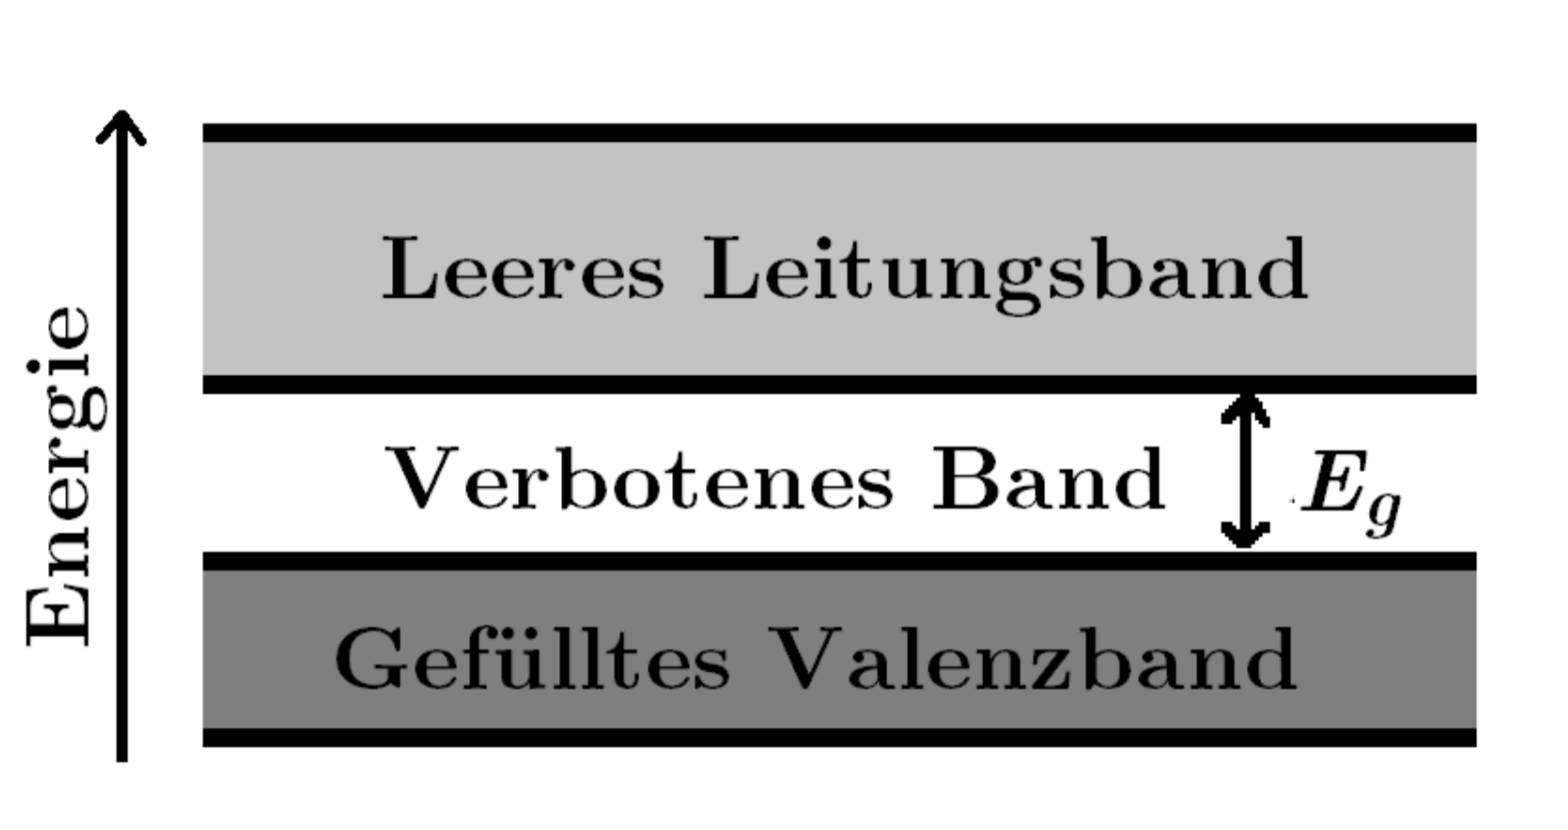
\includegraphics[height=6cm]{TimosAufrisse/bandmodell.png}
  \caption{Bandschema eines Halbleiters\cite{anleitung}.}
  \label{fig:bandmodell}
\end{figure}

Um die Leitfähigkeit von Halbleitern gezielt zu steigern werden sie mit Fremdatomen dotiert. Das hier verwendete Silizium besitzt vier Valenzelektronen. Nun wird hier Arsen als Donator mit fünf Valenzelektronen eingeführt. Dadurch ist ein Elektron nicht an der Bindung beteiligt und kann als Ladungsträger dienen. Außerdem kann noch Bor als Akzeptor mit drei Valenzelektronen eingeführt werden. So existiert eine elektronfreie Stelle ein Loch als Ladungsträger. Dargestellt ist dies in Abbildung \ref{fig:dotierung}.

\begin{figure}
  \centering
  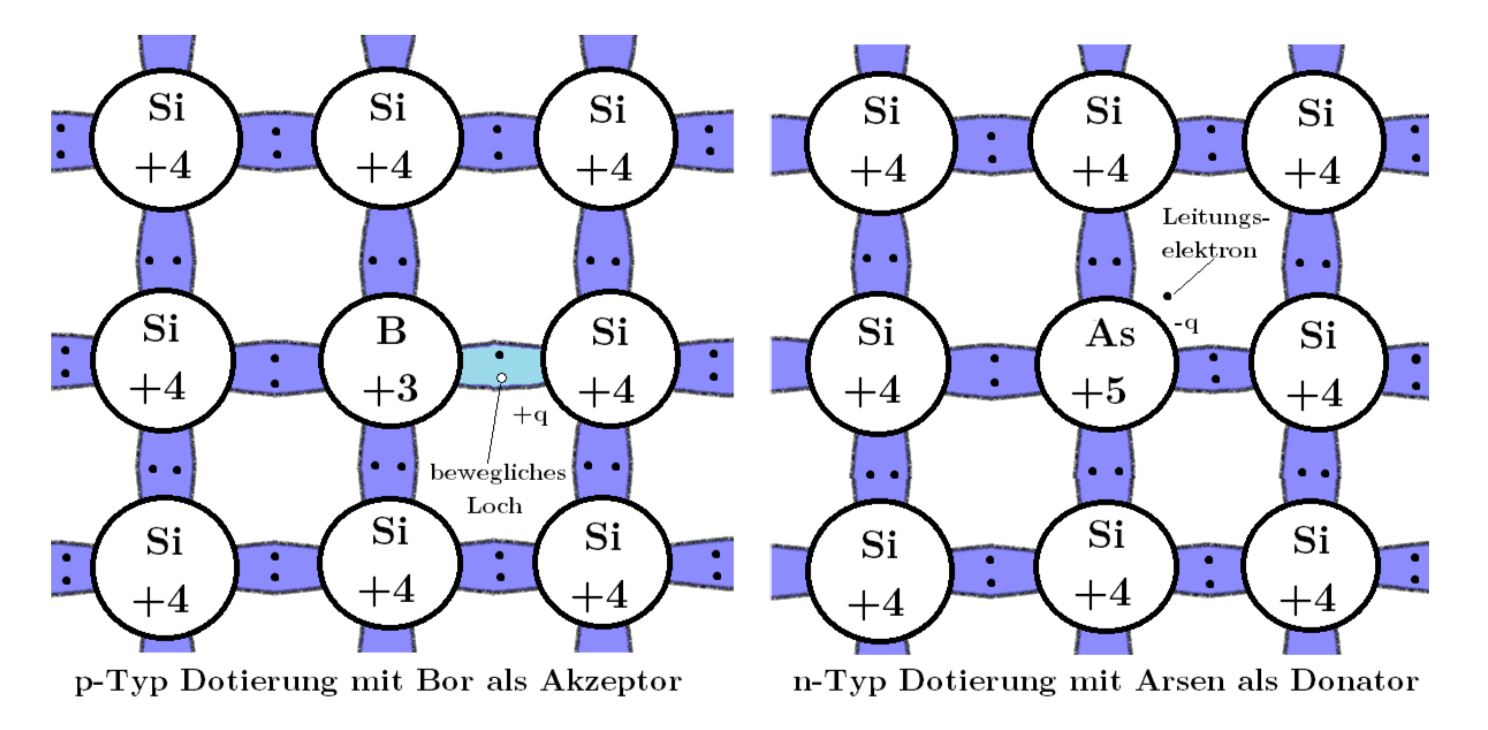
\includegraphics[height=6cm]{TimosAufrisse/dotierung.png}
  \caption{Skizze der zwei hier verwendeten Dotierungsarten \cite{anleitung}.}
  \label{fig:dotierung}
\end{figure}

Wenn ein mit Donatoren n-dotierter Halbleiter verbunden wird mit einem mit Akzeptoren p-dotierten bildet sich eine Depletionszone aus, da die freien Elektronen mit den Löchern kombinieren und so geladene Atomrümpfe hinterlassen. Dies ist in Abbildung \ref{fig:pnuebergang} zu sehen.

\begin{figure}
  \centering
  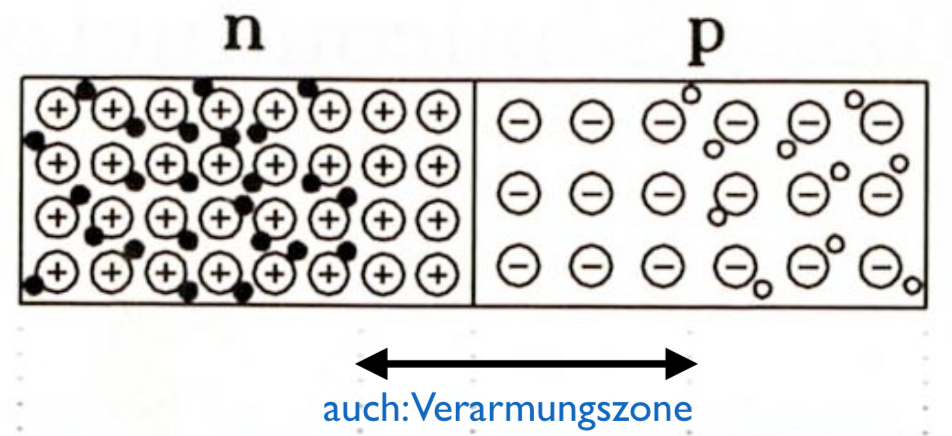
\includegraphics[height=4cm]{TimosAufrisse/pnuebergang.png}
  \caption{Darstellung der Verarmungszone bei einer Diode \cite{goessling}.}
  \label{fig:pnuebergang}
\end{figure}

% \subsection{Fehlerrechnung}
%
% Für die Fehlerfortpflanzung bei Gleichungen mit $N$ fehlerbehafteten Größen
% wird jeweils die Formel zur Gaußschen Fehlerfortpflanzung
%
% \begin{equation*}
%   \sigma = \sqrt{\sum_{i=1}^{N}\biggl(\frac{\partial f(x_{\g{i}})}{\partial x_{\g{i}}}
%   \sigma_{\g{i}}\biggr)^2}
% \end{equation*}
% mit der jeweiligen Funktion $f(x_{\g{i}})$, den Messgrößen $x_{\g{i}}$ und den
% zugehörigen Fehlern $\sigma_i$ verwendet.
% Zur Berechnung des arithmetischen Mittels von $N$ Messwerten wird jeweils die
% Formel
%
% \begin{equation*}
%   \bar{x} = \frac{1}{N}\sum_{i=1}^{N}x_{\g{i}}
% \end{equation*}
% mit den Messwerten $x_i$ benutzt.
% Die Standardabweichung des Mittelwerts wird jeweils mit der Gleichung
%
% \begin{equation*}
%   \bar{\sigma} = \sqrt{\frac{1}{N-1}\sum_{i=1}^{N}(x_{\g{i}} - \bar{x})^2}
% \end{equation*}
% mit den $N$ Messwerten $x_i$ berechnet.




\cite{anleitung}
